\begin{comment}	

The strange math.

\subsection{Backstory}
There was a conflict in russia, where Markow and X had different views an free will. 

Where 
marvo had the position, that random outcomes can be a result of depentend events.

Where X mad the flipped the inference, between:
indepented events $\rightarrow$ random outcomes
Concept of large numbers.

That independence of events are nessary to show the law of large numbers (merky).

Where X mad the flipp, when effects of large numbers are observed, then those mean, indpendenc of events are nessary - for him: free choice.

The senario is, total number of marrages. This percludes free choices, there for the hand of god. Who marrages whom. 

The senario: X observed social zufallsvariablen: yearly total number of mariage and other social statistics.

He observed, that those followed the law of large numbers. We resoned, that that means, that convergence of $\mu$ must mean, that the $X_i$ are indepented. This he set equal to, indiviual made indepente choices.

(Image for the flipped logic)

Inlcude: chapter_Mathematics/Scc001.

---

Marcov showed. That dependent events can produce convergens effects of large numbers.
\end{comment}

\chapter{Markov Chains}

\section{The Law of Large Numbers (LLN)}

The \textbf{Law of Large Numbers (LLN)} is a fundamental theorem in probability theory that describes how averages behave over many repetitions of a random experiment. It ensures that the average of repeated independent observations converges to the expected (theoretical) mean.

\subsection{Key Symbols}

\begin{center}
\begin{tabular}{ll}
\toprule
\textbf{Symbol} & \textbf{Meaning} \\
\midrule
$X_i$ & Random variable representing the $i$-th trial \\
$\mu = \mathbb{E}[X_i]$ & Expected (mean) value \\
$\overline{X}_n$ & Sample mean after $n$ observations \\
$\xrightarrow{P}$ & Convergence in probability \\
$\xrightarrow{\text{a.s.}}$ & Almost sure convergence \\
\bottomrule
\end{tabular}
\end{center}

\subsection{Setup}

Let
\[
\{X_1, X_2, \dots\}
\]
be a sequence of independent and identically distributed (i.i.d.) random variables with finite expected value
\[
\mathbb{E}[X_i] = \mu.
\]

Define the sample mean:
\[
\overline{X}_n = \frac{1}{n} \sum_{i=1}^{n} X_i.
\]

\subsection{Weak Law of Large Numbers (WLLN)}

The sample mean converges to the expected value \emph{in probability}:
\[
\overline{X}_n \xrightarrow{P} \mu \quad \text{as } n \to \infty,
\]
that is, for every $\varepsilon > 0$,
\[
\lim_{n \to \infty} \mathbb{P}(|\overline{X}_n - \mu| > \varepsilon) = 0.
\]

\subsection{Strong Law of Large Numbers (SLLN)}

The sample mean converges to $\mu$ \emph{almost surely}:
\[
\overline{X}_n \xrightarrow{\text{a.s.}} \mu \quad \text{as } n \to \infty,
\]
meaning
\[
\mathbb{P}\left( \lim_{n \to \infty} \overline{X}_n = \mu \right) = 1.
\]

\subsection{Interpretation}

The LLN justifies the use of empirical averages to estimate theoretical expectations. As the number of samples grows, randomness averages out, and the observed mean stabilizes around the true mean.



% ----------------------------------------------------------
\section{Markov Chains and Dependence}

\subsection{Key Symbols}


\begin{center}
\begin{tabular}{ll}
\toprule
\textbf{Symbol} & \textbf{Meaning} \\
\midrule
Markov property & $\,\mathbb{P}(X_{n+1}\!\mid X_n,\dots)=\mathbb{P}(X_{n+1}\!\mid X_n)$ (local forgetting) \\
Ergodicity & Global forgetting; convergence to a unique $\boldsymbol{\pi}$ \\
$\boldsymbol{\pi}$ & Stationary distribution ($\boldsymbol{\pi}P=\boldsymbol{\pi}$) \\
$S = \{s_1, \dots, s_k\}$ & Finite set of possible states \\
$X_n$ & State of the process at step $n$ \\
$\mathbb{P}(X_{n+1}=s_j \mid X_n=s_i)$ & Transition probability \\
\bottomrule
\end{tabular}
\end{center}


\subsection{Definition}

A \textbf{Markov chain} is a sequence of random variables
\[
X_1, X_2, X_3, \dots
\]
taking values in a state space
\[
S = \{ s_1, s_2, \dots, s_k \},
\]
and satisfying the \emph{Markov property}:
\[
\mathbb{P}(X_{n+1} = s_j \mid X_n = s_i, X_{n-1}, \dots, X_1)
= \mathbb{P}(X_{n+1} = s_j \mid X_n = s_i),
\quad \forall i,j.
\]

\subsection{Interpretation }

The \emph{Markov property} is a local forgetting statement: conditional on the
present state, the future is independent of the past. By itself, this property
does \emph{not} imply convergence of empirical averages.\\ 

However, if a Markov chain satisfies additional regularity conditions that
force \emph{global forgetting} (ergodicity)—for example, on a finite state space:
irreducibility, aperiodicity, and positive recurrence—then the chain admits a
unique stationary distribution $\boldsymbol{\pi}$, the law of $X_n$ converges to
$\boldsymbol{\pi}$ regardless of the start, and a Law of Large Numbers holds
for functions of the chain.\\

\textbf{In General:} Markov showed that independence is \emph{not necessary} for the Law of Large Numbers
to hold.  Even when consecutive events are dependent---as in a Markov chain---the
average value still converges to a stable limit if the dependence is sufficiently
regular (e.g., the chain is stationary or ergodic).  Thus, the LLN can be
``caused by dependent events.''

\begin{center}
\begin{tabular}{llll}
\toprule
\textbf{Case} & \textbf{Independence} & \textbf{Expectation} & \textbf{LLN Holds?} \\
\midrule
i.i.d. & Yes & Constant ($\mu$) & Yes \\
Stationary Markov Chain & No & Constant ($\mu$) & Yes \\
Ergodic Markov Chain & No & Converges to $\mu$ & Yes \\
\bottomrule
\end{tabular}
\end{center}


\noindent
In particular, independence of the $X_i$ is not necessary for an LLN:
what is needed is sufficient mixing/forgetting of the initial state, as
guaranteed by ergodicity.



%----- Missing: 

\section{Probability Distributions on Finite and Infinite State Spaces}

Let $S$ be the state space of a Markov chain. A \emph{probability distribution} on $S$
assigns to each state $i \in S$ a nonnegative number $\pi(i)$ representing the probability
that the chain is in state $i$, with the probabilities summing to one.

\subsection{Finite State Space.}
If the state space is finite,
\[
S = \{s_1, s_2, \dots, s_k\},
\]
then a probability distribution on $S$ is a vector
\[
\boldsymbol{\pi} = (\pi(s_1), \dots, \pi(s_k)),
\]
satisfying
\[
\pi(s_j) \ge 0, \qquad \sum_{j=1}^k \pi(s_j) = 1.
\]
In this case $\boldsymbol{\pi}$ is simply a finite probability vector.\\

The full probability distribution at time $n$.
The collection of all such probabilities,
\[
\boldsymbol{\pi}^{(n)} = 
\big( \mathbb{P}(X_n = s_1),\, \mathbb{P}(X_n = s_2),\, \dots \big),
\]
is the probability distribution of $X_n$.  Thus,
\[
\pi^{(n)}(j) = \mathbb{P}(X_n = s_j).
\]

\subsection{Countably Infinite State Space.}
If the state space is countably infinite,
\[
S = \{s_1, s_2, s_3, \dots\},
\]
then a probability distribution is an infinite sequence
\[
\boldsymbol{\pi} = (\pi(s_1), \pi(s_2), \ldots),
\]
satisfying
\[
\pi(s_j) \ge 0 \quad \text{for all } j, \qquad
\sum_{j=1}^{\infty} \pi(s_j) = 1.
\]
The normalization condition is now an infinite series, which must converge to 1.

\subsection{Interpretation}
In both cases, $\pi(i)$ gives the probability that $X_n = i$ when the chain is in
distribution $\boldsymbol{\pi}$. For finite state spaces the distribution is a finite
probability vector, while for infinite state spaces it is an infinite but summable
probability sequence.


\section{Evolution and Convergence}

\subsection{Key Symbols}

\begin{center}
\begin{tabular}{ll}
\toprule
\textbf{Symbol} & \textbf{Meaning} \\
\midrule
$P_{ij}$ & One-step transition probability \\
$P$ & Transition matrix \\
$P^n$ & $n$-step transition probabilities \\
Stationary $\boldsymbol{\pi}$ & Limiting equilibrium distribution \\
$\boldsymbol{\pi}^{(n)}$ & Distribution at step $n$ \\
$\boldsymbol{\pi}^{(0)}$ & Initial distribution vector \\
$\boldsymbol{\pi}$ & Stationary distribution \\
$\mu$ & Expected value under stationarity \\
\bottomrule
\end{tabular}
\end{center}

\subsection{Key Symbols - Transition Matrix}

\begin{center}
\begin{tabular}{ll}
\toprule
\textbf{Symbol} & \textbf{Meaning} \\
\midrule
$p_{VV}, p_{VC}, p_{CV}, p_{CC}$ & Transition probabilities \\
$\pi_V, \pi_C$ & Stationary probabilities \\
$\boldsymbol{\pi}^{(0)}$ & Initial distribution \\
$P^n$ & $n$-step transition matrix \\
\bottomrule
\end{tabular}
\end{center}


\subsection{Transition Matrix}

The one-step transition probabilities are collected into a matrix:
\[
P =
\begin{bmatrix}
P_{11} & P_{12} & \cdots & P_{1k} \\
P_{21} & P_{22} & \cdots & P_{2k} \\
\vdots & \vdots & \ddots & \vdots \\
P_{k1} & P_{k2} & \cdots & P_{kk}
\end{bmatrix}, \quad
\sum_{j=1}^{k} P_{ij} = 1.
\]
% ----------------------------------------------------------

\section{The Idea of Forgetting - Stationary and non-stationary Distributions}

\subsection{Key Symbols}

\begin{center}
\begin{tabular}{ll}
\toprule
\textbf{Symbol} & \textbf{Meaning} \\
\midrule
$P_{ij}$ & Probability of moving from state $s_i$ to $s_j$ \\
$\pi_j$ & Long-run (stationary) probability of state $s_j$ \\
$\boldsymbol{\pi}$ & Stationary distribution vector \\
Ergodic chain & Chain that “forgets” its start and converges to $\pi$ \\
\bottomrule
\end{tabular}
\end{center}

\subsection{Overview}

\begin{center}
\begin{tabular}{@{}llll@{}}
\toprule
\textbf{Case} & \textbf{Independence} & \textbf{Expectations} & \textbf{LLN holds?} \\
\midrule
i.i.d. & Yes & All equal ($\mathbb{E}[X_i] = \mu$) & Yes \\
Markov chain (stationary) & No & All equal ($\mathbb{E}[X_i] = \mu$) & Yes \\
Markov chain (ergodic) & No & Different initially, converge to $\mu$ & Yes \\
\bottomrule
\end{tabular}
\end{center}

\subsection{Stationary and Ergodic Chains}

A Markov chain is said to be \textbf{stationary} if its distribution does not
change with time:
\[
\mathbb{P}(X_{n+1} = j) = \mathbb{P}(X_n = j) \quad \forall n.
\]
In this case,
\[
\mathbb{E}[X_n] = \mathbb{E}[X_1] = \mu,
\]
and the Law of Large Numbers holds even though the $X_i$ are dependent:
\[
\frac{1}{n} \sum_{i=1}^{n} X_i \xrightarrow{\text{a.s.}} \mu.
\]

If the chain is not stationary but is \textbf{ergodic} (meaning it forgets its
initial state and converges to a unique stationary distribution), then
\[
\mathbb{E}[X_i] \to \mu \quad \text{as } i \to \infty,
\]
and the sample average still satisfies
\[
\frac{1}{n} \sum_{i=1}^{n} X_i \xrightarrow{\text{a.s.}} \mu.
\]

\subsection{Stationary Chain}
A probability distribution $\boldsymbol{\pi}$ on the state space $S$ is called a
\emph{stationary distribution} of a Markov chain with transition matrix $P$ if,
when the chain starts with initial distribution $\boldsymbol{\pi}^{(0)} =
\boldsymbol{\pi}$, the distribution remains unchanged at all future times. That is,
\[
\boldsymbol{\pi}^{(n)} = \boldsymbol{\pi} \quad \text{for all } n \ge 0.
\]

Using the evolution equation $\boldsymbol{\pi}^{(n+1)} = \boldsymbol{\pi}^{(n)} P$,
this condition is equivalent to the requirement
\[
\boldsymbol{\pi} = \boldsymbol{\pi}P,
\]
or, componentwise,
\[
\pi(j) = \sum_{i \in S} \pi(i) P(i,j), \qquad j \in S.
\]

Thus a stationary distribution is one that, when used as the initial law of the
Markov chain, remains invariant under the dynamics: the chain started in
$\boldsymbol{\pi}$ stays in $\boldsymbol{\pi}$ for all time.





\subsection{Ergodic Chains}

Even if the initial distribution is non-stationary, an \textbf{ergodic} chain converges to a unique stationary distribution:
\[
\boldsymbol{\pi}^{(n)} = \boldsymbol{\pi}^{(0)} P^n \to \boldsymbol{\pi}.
\]
Thus, the Law of Large Numbers still holds:
\[
\frac{1}{n} \sum_{i=1}^{n} X_i \xrightarrow{\text{a.s.}} \mu.
\]


\subsection{Local Forgetting}

The \textbf{Markov property} expresses local forgetting:
\[
\mathbb{P}(X_{n+1} = x_{n+1} \mid X_n = x_n, X_{n-1}, \dots)
= \mathbb{P}(X_{n+1} = x_{n+1} \mid X_n = x_n).
\]
Once the current state is known, the past is irrelevant.

\subsection{Global Forgetting (Ergodicity)}

In many chains, as $n \to \infty$, the effect of the initial state vanishes:
\[
\lim_{n \to \infty} \mathbb{P}(X_n = s_j \mid X_0 = s_i) = \pi_j,
\]
where $\boldsymbol{\pi} = (\pi_1, \dots, \pi_k)$ is the \emph{stationary distribution}, independent of the start.



% ----------------------------------------------------------

\subsection{Evolution Equation}

The evolution of state probabilities is governed by:
\[
\boldsymbol{\pi}^{(n+1)} = \boldsymbol{\pi}^{(n)} P, \quad
\boldsymbol{\pi}^{(n)} = \boldsymbol{\pi}^{(0)} P^n.
\]

Different initial distributions (e.g., all vowels, all consonants, or mixed) will all converge to the same stationary distribution in ergodic chains.




% ----------------------------------------------------------
\section{Example: Two-State Markov Chain - Vowel Constant}




\subsection{Setup}

\[
S = \{V, C\}, \quad
P =
\begin{bmatrix}
p_{VV} & p_{VC} \\
p_{CV} & p_{CC}
\end{bmatrix},
\quad
p_{VC} = 1 - p_{VV}, \quad
p_{CV} = 1 - p_{CC}.
\]

The stationary distribution $\boldsymbol{\pi} = [\pi_V, \pi_C]$ satisfies:

\[
\begin{cases}
\pi_V = \pi_V p_{VV} + \pi_C p_{CV}, \\
\pi_C = \pi_V p_{VC} + \pi_C p_{CC}, \\
\boldsymbol{\pi} P = \boldsymbol{\pi},\\ 
\pi_V + \pi_C = 1.
\end{cases}
\]

\subsection{Three differente Transition Probablity representation}

Consider a simple two-state system:
\[
S = \{V, C\},
\]
where $V$ represents a vowel and $C$ a consonant. The transitions are given by
\[
\mathbb{P}(X_{n+1}=V \mid X_n=V) = 0.8, \quad
\mathbb{P}(X_{n+1}=C \mid X_n=V) = 0.2,
\]
\[
\mathbb{P}(X_{n+1}=V \mid X_n=C) = 0.4, \quad
\mathbb{P}(X_{n+1}=C \mid X_n=C) = 0.6.
\]

or represented in matrix form

\[
P =
\begin{bmatrix}
0.8 & 0.2 \\
0.4 & 0.6
\end{bmatrix}.
\]

or represented in transition diagramm
\begin{figure}[htbp]
\centering
\begin{tikzpicture}[
    scale=1.2,
    transform shape,
    ->, >=Stealth,
    node distance=2cm,
    font=\large,
    every edge/.style={draw, thick, black}
]

% Define node styles
\tikzset{
    vowel/.style={
        circle,
        draw=orange!90!black,
        very thick,
        minimum size=1cm,
        text=orange!90!black,
        font=\bfseries\Large,
        align=center
    },
    consonant/.style={
        circle,
        draw=blue!80!black,
        very thick,
        minimum size=1cm,
        text=blue!80!black,
        font=\bfseries\Large,
        align=center
    }
}

% Nodes
\node[vowel] (V) {V};
\node[consonant, right of=V] (C) {C};

% Self-loops
\path (V) edge[loop left, min distance=10mm, in=210, out=150]
    node[left=3pt] {$p_{VV}= 0.80$} (V);
\path (C) edge[loop right, min distance=10mm, in=30, out=-30]
    node[right=3pt] {$p_{CC}= 0.60$} (C);

% Cross transitions
\path (V) edge[bend left=90] node[above] {$p_{VC}= 0.20$} (C);
\path (C) edge[bend left=90] node[below] {$p_{CV}= 0.40$} (V);

\end{tikzpicture}
\caption{Vowel–Consonant Transition Diagram}
\label{fig:vowel-consonant-diagram}
\end{figure}

If the current state is a vowel ($X_n = V$), the probability of the next state being 
a vowel is always $0.8$, no matter how we reached the current vowel. Whether the 
previous sequence was ``CVCV'' or ``VVVV'' does not change the probability of the 
next step. Thus, only the \emph{current state} matters for predicting the next one.


\subsection{Interation}
\subsubsection{One}
The probability of transitioning depends only on the current state—how we got there is 




\[
P =
\begin{bmatrix}
0.8 & 0.2 \\
0.4 & 0.6
\end{bmatrix}
\Rightarrow
\boldsymbol{\pi} = [0.667, 0.333].
\]

Thus, vowels occur about $2/3$ of the time, consonants $1/3$, regardless of the starting state.


\subsubsection{Converging}

The initial vector $\boldsymbol{\pi}^{(0)}$ represents the probabilities of starting in each state.  
It can be any valid probability distribution (summing to 1), for example:

\begin{center}
\begin{tabular}{@{}lll@{}}
\toprule
\textbf{Starting condition} & \textbf{Initial vector $\boldsymbol{\pi}^{(0)}$} & \textbf{Meaning} \\ \midrule
All vowels & $[1,\, 0]$ & Certain start in $V$ \\
All consonants & $[0,\, 1]$ & Certain start in $C$ \\
Half vowels, half consonants & $[0.5,\, 0.5]$ & Mixed random start \\
30\% vowels, 70\% consonants & $[0.3,\, 0.7]$ & Biased random start \\
\bottomrule
\end{tabular}
\end{center}

Each of these starting distributions evolves over time according to
\[
\boldsymbol{\pi}^{(n)} = \boldsymbol{\pi}^{(0)} P^n.
\]

For example:
\[
\begin{aligned}
\text{If } \boldsymbol{\pi}^{(0)} &= [1, 0], & \boldsymbol{\pi}^{(1)} &= [0.8, 0.2], & \boldsymbol{\pi}^{(2)} &= [0.72, 0.28], \\
\text{If } \boldsymbol{\pi}^{(0)} &= [0, 1], & \boldsymbol{\pi}^{(1)} &= [0.4, 0.6], & \boldsymbol{\pi}^{(2)} &= [0.56, 0.44].
\end{aligned}
\]

Although they start differently, both sequences converge to the same long-run equilibrium.

\subsubsection{Visualization of Convergence (``Forgetting'')}

For the matrix above,
\[
\boldsymbol{\pi} = [0.667, 0.333].
\]
That means that, in the long run, the process will be in vowels about 66.7\% of the time and in consonants about 33.3\% of the time.



\begin{center}
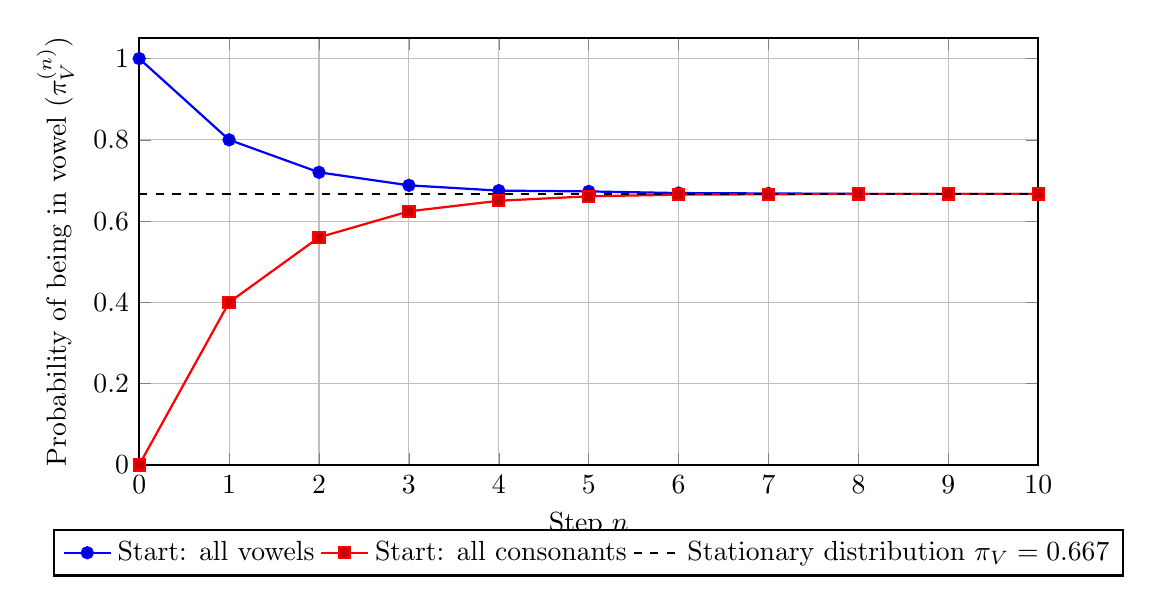
\begin{tikzpicture}
\begin{axis}[
    width=13cm, height=7cm,
    xlabel={Step $n$},
    ylabel={Probability of being in vowel ($\pi_V^{(n)}$)},
    xmin=0, xmax=10,
    ymin=0.0, ymax=1.05,
    grid=major,
    thick,
    legend style={at={(0.5,-0.15)}, anchor=north, legend columns=-1}
]

% Starting from all vowels
\addplot+[mark=*] coordinates {
(0, 1.000)
(1, 0.800)
(2, 0.720)
(3, 0.688)
(4, 0.675)
(5, 0.673)
(6, 0.669)
(7, 0.668)
(8, 0.667)
(9, 0.667)
(10, 0.667)
};
\addlegendentry{Start: all vowels}

% Starting from all consonants
\addplot+[mark=square*] coordinates {
(0, 0.000)
(1, 0.400)
(2, 0.560)
(3, 0.624)
(4, 0.650)
(5, 0.661)
(6, 0.665)
(7, 0.666)
(8, 0.667)
(9, 0.667)
(10, 0.667)
};
\addlegendentry{Start: all consonants}

% Stationary distribution line
\addplot[dashed, domain=0:10, samples=2] {0.667};
\addlegendentry{Stationary distribution $\pi_V = 0.667$}

\end{axis}
\end{tikzpicture}
\end{center}

\subsection{Interpretation}

This plot shows how different initial starting conditions lead to the same long-run behavior.
Even though one chain begins entirely in vowels and the other entirely in consonants,
both converge to the same stationary distribution.
This illustrates the \emph{forgetting property} of Markov chains:
the system ``forgets'' its initial state and stabilizes in equilibrium.



% ----------------------------------------------------------
